\documentclass[12pt]{article}

\usepackage[margin=1in]{geometry} 
\usepackage{amsmath,amsthm,amssymb}
\usepackage[spanish]{babel}
\usepackage[utf8]{inputenc}
\usepackage{tikz-cd}
\usepackage{amsmath}
\usepackage[shortlabels]{enumitem}
\usepackage{mathtools}
\usepackage{float}
\usepackage{listings}

\begin{document}

\title{SWAP: Ejercicios T4 Opcionales}
\author{
        Antonio Gámiz Delgado
}
\maketitle
\medskip

\section{Ejercicio T4.5}
\textbf{Enunciado:} Implementar un pequeño servicio web en los servidores finales que devuelva el \% CPU y \% RAM que en un instante tiene en uso dicho servidor. Lo debe devolver como una cadena de texto plano que representa ambos porcentajes: 'CPU 45\% RAM 76\%'.

Este ejercicio lo vamos a realizar en \textit{M1}. Creamos un script para obtener el string deseado:

\begin{figure}[H]
  \center
  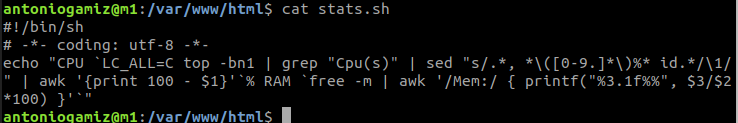
\includegraphics[scale=0.5]{img/1.png}
\end{figure}

Creamos un archivo php para ejecutar ese script y que devuelva el resultado:

\begin{figure}[H]
  \center
  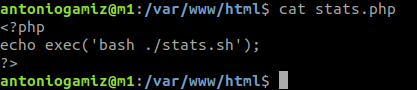
\includegraphics[scale=0.5]{img/2.png}
\end{figure}

Comprobamos que funciona correctamente:

\begin{figure}[H]
  \center
  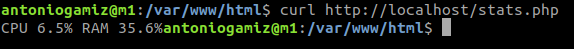
\includegraphics[scale=0.5]{img/3.png}
\end{figure}

\newpage

\section{Ejercicio T4.7}
\textbf{Enunciado:} Probar las diferentes maneras de redirección HTTP. ¿Cuál es la adecuada y cuál no lo es para hacer balanceo de carga global? ¿Por qué?
\section{Ejercicio T4.8}
\textbf{Enunciado:} Buscar información sobre los bloques de IP para los distintos países o continentes. Implementar en JavaScript o PHP la detección de la zona desde donde se conecta un usuario.

Primero necesitamos descargarnos una lista de IPs por país para poder clasificarla, lo podemos hacer en \cite{d}. Como está en formato CSV, instalamos un parser para usarlo en JS:

\begin{figure}[H]
  \center
  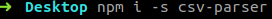
\includegraphics[scale=0.5]{img/4.png}
\end{figure}

Una vez instalado, creamos un programa en JS para que compare los 3 primeros octetos de la IP (todos tienen máscara 24):

\begin{figure}[H]
  \center
  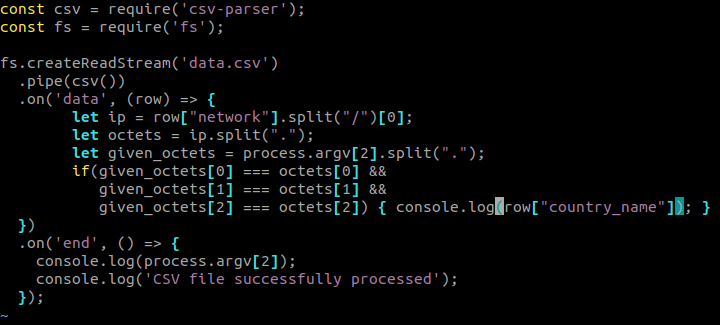
\includegraphics[scale=0.5]{img/5.png}
\end{figure}

Ejecutamos el programa y le pasamos una IP de prueba:

\begin{figure}[H]
  \center
  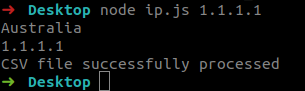
\includegraphics[scale=0.5]{img/6.png}
\end{figure}

\begin{thebibliography}{9}
\bibitem{c}
https://askubuntu.com/questions/941949/one-liner-to-show-cpu-ram-and-hdd-usage
\bibitem{d}
https://lite.ip2location.com/ip-address-ranges-by-country
\bibitem{a}
https://stackabuse.com/reading-and-writing-csv-files-with-node-js/
\end{thebibliography}

%\begin{figure}[H]
%  \center
%  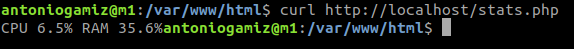
\includegraphics[scale=0.5]{img/3.png}
%\end{figure}

\end{document}
